% FridgeMoCA V3 Architecture Diagram
% Include with: % FridgeMoCA V3 Architecture Diagram
% Include with: % FridgeMoCA V3 Architecture Diagram
% Include with: % FridgeMoCA V3 Architecture Diagram
% Include with: \input{figures/architecture.tex}
% Requires: \usepackage{tikz}

\begin{figure}[ht]
\centering
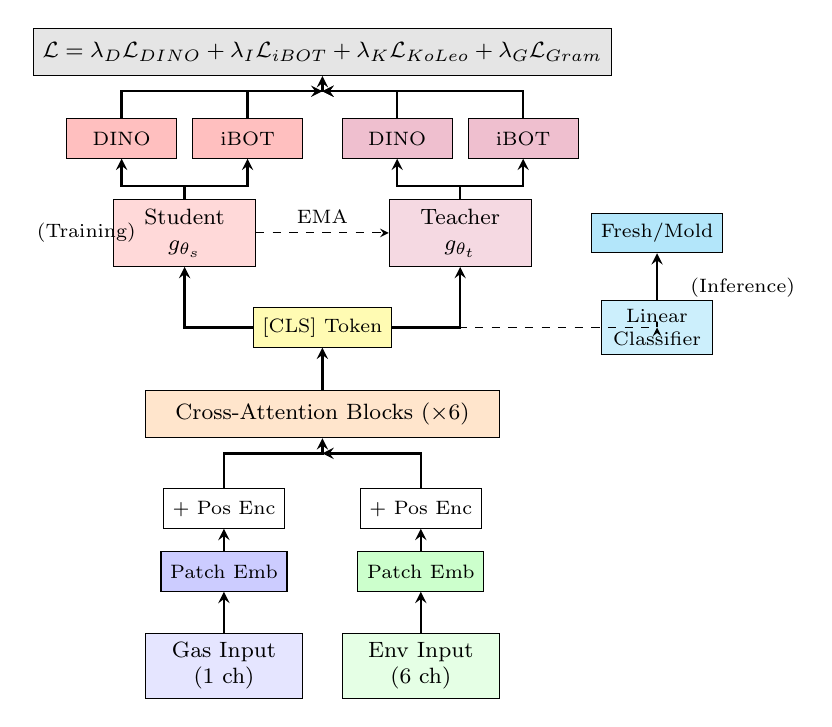
\begin{tikzpicture}[
    node distance=0.8cm,
    box/.style={rectangle, draw, minimum width=2cm, minimum height=0.6cm, align=center, font=\footnotesize},
    smallbox/.style={rectangle, draw, minimum width=1.4cm, minimum height=0.5cm, align=center, font=\scriptsize},
    arrow/.style={->, >=stealth, thick},
    dashedarrow/.style={->, >=stealth, dashed},
    label/.style={font=\scriptsize}
]

% Input
\node[box, fill=blue!10] (gas) at (0, 0) {Gas Input\\(1 ch)};
\node[box, fill=green!10] (env) at (2.5, 0) {Env Input\\(6 ch)};

% Patch Embedding
\node[smallbox, fill=blue!20] (gasemb) at (0, 1.2) {Patch Emb};
\node[smallbox, fill=green!20] (envemb) at (2.5, 1.2) {Patch Emb};

% Positional Encoding
\node[smallbox] (gaspos) at (0, 2.0) {+ Pos Enc};
\node[smallbox] (envpos) at (2.5, 2.0) {+ Pos Enc};

% Cross Attention Blocks
\node[box, fill=orange!20, minimum width=4.5cm] (transformer) at (1.25, 3.2) {Cross-Attention Blocks ($\times$6)};

% CLS Token
\node[smallbox, fill=yellow!30] (cls) at (1.25, 4.3) {[CLS] Token};

% Split into Student/Teacher
\node[box, fill=red!15, minimum width=1.8cm] (student) at (-0.5, 5.5) {Student\\$g_{\theta_s}$};
\node[box, fill=purple!15, minimum width=1.8cm] (teacher) at (3.0, 5.5) {Teacher\\$g_{\theta_t}$};

% Projection Heads
\node[smallbox, fill=red!25] (dinohead) at (-1.3, 6.7) {DINO};
\node[smallbox, fill=red!25] (ibothead) at (0.3, 6.7) {iBOT};
\node[smallbox, fill=purple!25] (tdinohead) at (2.2, 6.7) {DINO};
\node[smallbox, fill=purple!25] (tibothead) at (3.8, 6.7) {iBOT};

% Losses
\node[box, fill=gray!20, minimum width=4.5cm] (loss) at (1.25, 7.8) {$\mathcal{L} = \lambda_D\mathcal{L}_{DINO} + \lambda_I\mathcal{L}_{iBOT} + \lambda_K\mathcal{L}_{KoLeo} + \lambda_G\mathcal{L}_{Gram}$};

% Classifier (inference)
\node[smallbox, fill=cyan!20] (classifier) at (5.5, 4.3) {Linear\\Classifier};
\node[smallbox, fill=cyan!30] (output) at (5.5, 5.5) {Fresh/Mold};

% Arrows - Input to Embedding
\draw[arrow] (gas) -- (gasemb);
\draw[arrow] (env) -- (envemb);

% Arrows - Embedding to Pos
\draw[arrow] (gasemb) -- (gaspos);
\draw[arrow] (envemb) -- (envpos);

% Arrows - Pos to Transformer
\draw[arrow] (gaspos) -- (0, 2.7) -- (1.25, 2.7) -- (transformer);
\draw[arrow] (envpos) -- (2.5, 2.7) -- (1.25, 2.7);

% Transformer to CLS
\draw[arrow] (transformer) -- (cls);

% CLS to Student/Teacher
\draw[arrow] (cls) -- (-0.5, 4.3) -- (student);
\draw[arrow] (cls) -- (3.0, 4.3) -- (teacher);

% Student to heads
\draw[arrow] (student) -- (-0.5, 6.1) -- (-1.3, 6.1) -- (dinohead);
\draw[arrow] (student) -- (-0.5, 6.1) -- (0.3, 6.1) -- (ibothead);

% Teacher to heads
\draw[arrow] (teacher) -- (3.0, 6.1) -- (2.2, 6.1) -- (tdinohead);
\draw[arrow] (teacher) -- (3.0, 6.1) -- (3.8, 6.1) -- (tibothead);

% Heads to Loss
\draw[arrow] (dinohead) -- (-1.3, 7.3) -- (1.25, 7.3) -- (loss);
\draw[arrow] (ibothead) -- (0.3, 7.3) -- (1.25, 7.3);
\draw[arrow] (tdinohead) -- (2.2, 7.3) -- (1.25, 7.3);
\draw[arrow] (tibothead) -- (3.8, 7.3) -- (1.25, 7.3);

% EMA arrow
\draw[dashedarrow] (student.east) -- node[above, label] {EMA} (teacher.west);

% Classifier branch
\draw[dashedarrow] (cls) -- (5.5, 4.3) -- (classifier);
\draw[arrow] (classifier) -- (output);

% Labels
\node[label, anchor=west] at (5.8, 4.8) {(Inference)};
\node[label, anchor=west] at (-2.5, 5.5) {(Training)};

\end{tikzpicture}
\caption{FridgeMoCA V3 architecture. During training, a student-teacher framework with EMA updates learns representations via DINO and iBOT objectives. At inference, only the student encoder and a frozen linear classifier are used.}
\label{fig:architecture}
\end{figure}

% Requires: \usepackage{tikz}

\begin{figure}[ht]
\centering
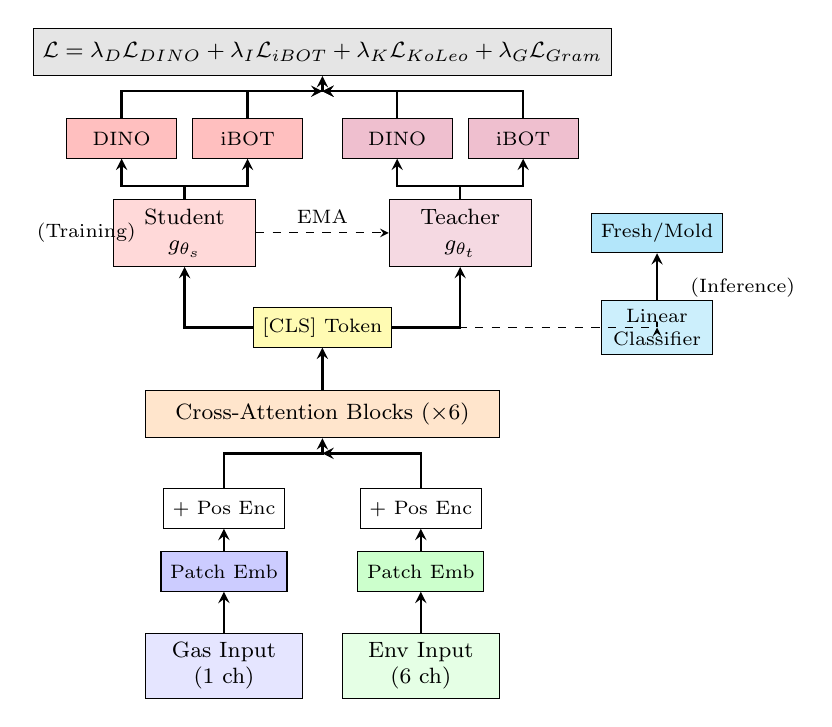
\begin{tikzpicture}[
    node distance=0.8cm,
    box/.style={rectangle, draw, minimum width=2cm, minimum height=0.6cm, align=center, font=\footnotesize},
    smallbox/.style={rectangle, draw, minimum width=1.4cm, minimum height=0.5cm, align=center, font=\scriptsize},
    arrow/.style={->, >=stealth, thick},
    dashedarrow/.style={->, >=stealth, dashed},
    label/.style={font=\scriptsize}
]

% Input
\node[box, fill=blue!10] (gas) at (0, 0) {Gas Input\\(1 ch)};
\node[box, fill=green!10] (env) at (2.5, 0) {Env Input\\(6 ch)};

% Patch Embedding
\node[smallbox, fill=blue!20] (gasemb) at (0, 1.2) {Patch Emb};
\node[smallbox, fill=green!20] (envemb) at (2.5, 1.2) {Patch Emb};

% Positional Encoding
\node[smallbox] (gaspos) at (0, 2.0) {+ Pos Enc};
\node[smallbox] (envpos) at (2.5, 2.0) {+ Pos Enc};

% Cross Attention Blocks
\node[box, fill=orange!20, minimum width=4.5cm] (transformer) at (1.25, 3.2) {Cross-Attention Blocks ($\times$6)};

% CLS Token
\node[smallbox, fill=yellow!30] (cls) at (1.25, 4.3) {[CLS] Token};

% Split into Student/Teacher
\node[box, fill=red!15, minimum width=1.8cm] (student) at (-0.5, 5.5) {Student\\$g_{\theta_s}$};
\node[box, fill=purple!15, minimum width=1.8cm] (teacher) at (3.0, 5.5) {Teacher\\$g_{\theta_t}$};

% Projection Heads
\node[smallbox, fill=red!25] (dinohead) at (-1.3, 6.7) {DINO};
\node[smallbox, fill=red!25] (ibothead) at (0.3, 6.7) {iBOT};
\node[smallbox, fill=purple!25] (tdinohead) at (2.2, 6.7) {DINO};
\node[smallbox, fill=purple!25] (tibothead) at (3.8, 6.7) {iBOT};

% Losses
\node[box, fill=gray!20, minimum width=4.5cm] (loss) at (1.25, 7.8) {$\mathcal{L} = \lambda_D\mathcal{L}_{DINO} + \lambda_I\mathcal{L}_{iBOT} + \lambda_K\mathcal{L}_{KoLeo} + \lambda_G\mathcal{L}_{Gram}$};

% Classifier (inference)
\node[smallbox, fill=cyan!20] (classifier) at (5.5, 4.3) {Linear\\Classifier};
\node[smallbox, fill=cyan!30] (output) at (5.5, 5.5) {Fresh/Mold};

% Arrows - Input to Embedding
\draw[arrow] (gas) -- (gasemb);
\draw[arrow] (env) -- (envemb);

% Arrows - Embedding to Pos
\draw[arrow] (gasemb) -- (gaspos);
\draw[arrow] (envemb) -- (envpos);

% Arrows - Pos to Transformer
\draw[arrow] (gaspos) -- (0, 2.7) -- (1.25, 2.7) -- (transformer);
\draw[arrow] (envpos) -- (2.5, 2.7) -- (1.25, 2.7);

% Transformer to CLS
\draw[arrow] (transformer) -- (cls);

% CLS to Student/Teacher
\draw[arrow] (cls) -- (-0.5, 4.3) -- (student);
\draw[arrow] (cls) -- (3.0, 4.3) -- (teacher);

% Student to heads
\draw[arrow] (student) -- (-0.5, 6.1) -- (-1.3, 6.1) -- (dinohead);
\draw[arrow] (student) -- (-0.5, 6.1) -- (0.3, 6.1) -- (ibothead);

% Teacher to heads
\draw[arrow] (teacher) -- (3.0, 6.1) -- (2.2, 6.1) -- (tdinohead);
\draw[arrow] (teacher) -- (3.0, 6.1) -- (3.8, 6.1) -- (tibothead);

% Heads to Loss
\draw[arrow] (dinohead) -- (-1.3, 7.3) -- (1.25, 7.3) -- (loss);
\draw[arrow] (ibothead) -- (0.3, 7.3) -- (1.25, 7.3);
\draw[arrow] (tdinohead) -- (2.2, 7.3) -- (1.25, 7.3);
\draw[arrow] (tibothead) -- (3.8, 7.3) -- (1.25, 7.3);

% EMA arrow
\draw[dashedarrow] (student.east) -- node[above, label] {EMA} (teacher.west);

% Classifier branch
\draw[dashedarrow] (cls) -- (5.5, 4.3) -- (classifier);
\draw[arrow] (classifier) -- (output);

% Labels
\node[label, anchor=west] at (5.8, 4.8) {(Inference)};
\node[label, anchor=west] at (-2.5, 5.5) {(Training)};

\end{tikzpicture}
\caption{FridgeMoCA V3 architecture. During training, a student-teacher framework with EMA updates learns representations via DINO and iBOT objectives. At inference, only the student encoder and a frozen linear classifier are used.}
\label{fig:architecture}
\end{figure}

% Requires: \usepackage{tikz}

\begin{figure}[ht]
\centering
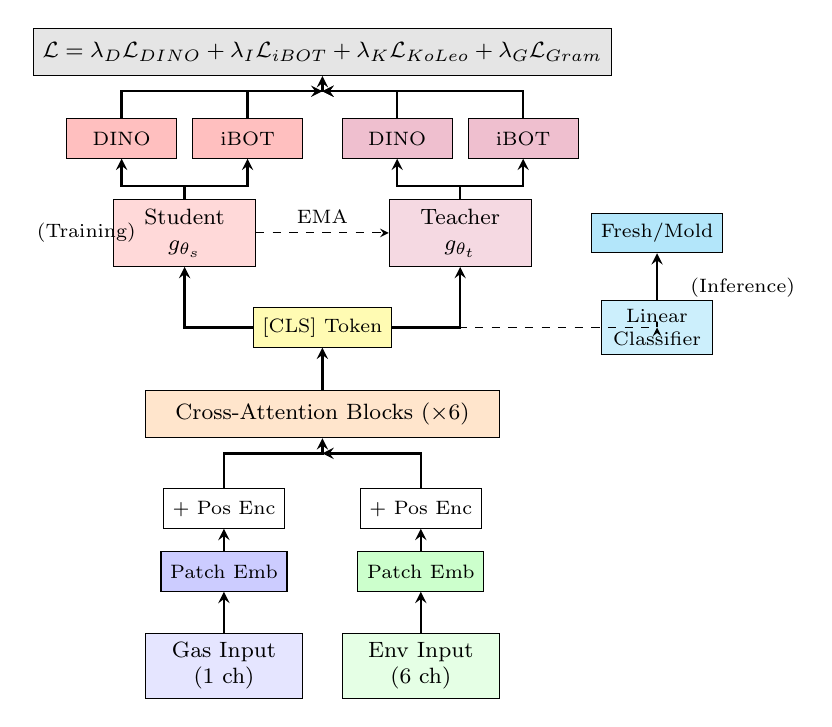
\begin{tikzpicture}[
    node distance=0.8cm,
    box/.style={rectangle, draw, minimum width=2cm, minimum height=0.6cm, align=center, font=\footnotesize},
    smallbox/.style={rectangle, draw, minimum width=1.4cm, minimum height=0.5cm, align=center, font=\scriptsize},
    arrow/.style={->, >=stealth, thick},
    dashedarrow/.style={->, >=stealth, dashed},
    label/.style={font=\scriptsize}
]

% Input
\node[box, fill=blue!10] (gas) at (0, 0) {Gas Input\\(1 ch)};
\node[box, fill=green!10] (env) at (2.5, 0) {Env Input\\(6 ch)};

% Patch Embedding
\node[smallbox, fill=blue!20] (gasemb) at (0, 1.2) {Patch Emb};
\node[smallbox, fill=green!20] (envemb) at (2.5, 1.2) {Patch Emb};

% Positional Encoding
\node[smallbox] (gaspos) at (0, 2.0) {+ Pos Enc};
\node[smallbox] (envpos) at (2.5, 2.0) {+ Pos Enc};

% Cross Attention Blocks
\node[box, fill=orange!20, minimum width=4.5cm] (transformer) at (1.25, 3.2) {Cross-Attention Blocks ($\times$6)};

% CLS Token
\node[smallbox, fill=yellow!30] (cls) at (1.25, 4.3) {[CLS] Token};

% Split into Student/Teacher
\node[box, fill=red!15, minimum width=1.8cm] (student) at (-0.5, 5.5) {Student\\$g_{\theta_s}$};
\node[box, fill=purple!15, minimum width=1.8cm] (teacher) at (3.0, 5.5) {Teacher\\$g_{\theta_t}$};

% Projection Heads
\node[smallbox, fill=red!25] (dinohead) at (-1.3, 6.7) {DINO};
\node[smallbox, fill=red!25] (ibothead) at (0.3, 6.7) {iBOT};
\node[smallbox, fill=purple!25] (tdinohead) at (2.2, 6.7) {DINO};
\node[smallbox, fill=purple!25] (tibothead) at (3.8, 6.7) {iBOT};

% Losses
\node[box, fill=gray!20, minimum width=4.5cm] (loss) at (1.25, 7.8) {$\mathcal{L} = \lambda_D\mathcal{L}_{DINO} + \lambda_I\mathcal{L}_{iBOT} + \lambda_K\mathcal{L}_{KoLeo} + \lambda_G\mathcal{L}_{Gram}$};

% Classifier (inference)
\node[smallbox, fill=cyan!20] (classifier) at (5.5, 4.3) {Linear\\Classifier};
\node[smallbox, fill=cyan!30] (output) at (5.5, 5.5) {Fresh/Mold};

% Arrows - Input to Embedding
\draw[arrow] (gas) -- (gasemb);
\draw[arrow] (env) -- (envemb);

% Arrows - Embedding to Pos
\draw[arrow] (gasemb) -- (gaspos);
\draw[arrow] (envemb) -- (envpos);

% Arrows - Pos to Transformer
\draw[arrow] (gaspos) -- (0, 2.7) -- (1.25, 2.7) -- (transformer);
\draw[arrow] (envpos) -- (2.5, 2.7) -- (1.25, 2.7);

% Transformer to CLS
\draw[arrow] (transformer) -- (cls);

% CLS to Student/Teacher
\draw[arrow] (cls) -- (-0.5, 4.3) -- (student);
\draw[arrow] (cls) -- (3.0, 4.3) -- (teacher);

% Student to heads
\draw[arrow] (student) -- (-0.5, 6.1) -- (-1.3, 6.1) -- (dinohead);
\draw[arrow] (student) -- (-0.5, 6.1) -- (0.3, 6.1) -- (ibothead);

% Teacher to heads
\draw[arrow] (teacher) -- (3.0, 6.1) -- (2.2, 6.1) -- (tdinohead);
\draw[arrow] (teacher) -- (3.0, 6.1) -- (3.8, 6.1) -- (tibothead);

% Heads to Loss
\draw[arrow] (dinohead) -- (-1.3, 7.3) -- (1.25, 7.3) -- (loss);
\draw[arrow] (ibothead) -- (0.3, 7.3) -- (1.25, 7.3);
\draw[arrow] (tdinohead) -- (2.2, 7.3) -- (1.25, 7.3);
\draw[arrow] (tibothead) -- (3.8, 7.3) -- (1.25, 7.3);

% EMA arrow
\draw[dashedarrow] (student.east) -- node[above, label] {EMA} (teacher.west);

% Classifier branch
\draw[dashedarrow] (cls) -- (5.5, 4.3) -- (classifier);
\draw[arrow] (classifier) -- (output);

% Labels
\node[label, anchor=west] at (5.8, 4.8) {(Inference)};
\node[label, anchor=west] at (-2.5, 5.5) {(Training)};

\end{tikzpicture}
\caption{FridgeMoCA V3 architecture. During training, a student-teacher framework with EMA updates learns representations via DINO and iBOT objectives. At inference, only the student encoder and a frozen linear classifier are used.}
\label{fig:architecture}
\end{figure}

% Requires: \usepackage{tikz}

\begin{figure}[ht]
\centering
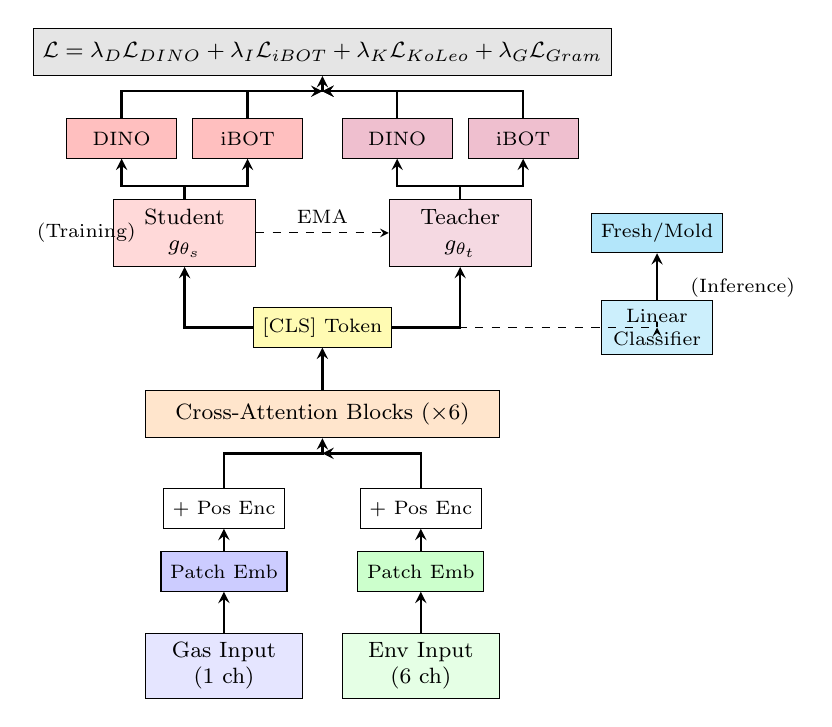
\begin{tikzpicture}[
    node distance=0.8cm,
    box/.style={rectangle, draw, minimum width=2cm, minimum height=0.6cm, align=center, font=\footnotesize},
    smallbox/.style={rectangle, draw, minimum width=1.4cm, minimum height=0.5cm, align=center, font=\scriptsize},
    arrow/.style={->, >=stealth, thick},
    dashedarrow/.style={->, >=stealth, dashed},
    label/.style={font=\scriptsize}
]

% Input
\node[box, fill=blue!10] (gas) at (0, 0) {Gas Input\\(1 ch)};
\node[box, fill=green!10] (env) at (2.5, 0) {Env Input\\(6 ch)};

% Patch Embedding
\node[smallbox, fill=blue!20] (gasemb) at (0, 1.2) {Patch Emb};
\node[smallbox, fill=green!20] (envemb) at (2.5, 1.2) {Patch Emb};

% Positional Encoding
\node[smallbox] (gaspos) at (0, 2.0) {+ Pos Enc};
\node[smallbox] (envpos) at (2.5, 2.0) {+ Pos Enc};

% Cross Attention Blocks
\node[box, fill=orange!20, minimum width=4.5cm] (transformer) at (1.25, 3.2) {Cross-Attention Blocks ($\times$6)};

% CLS Token
\node[smallbox, fill=yellow!30] (cls) at (1.25, 4.3) {[CLS] Token};

% Split into Student/Teacher
\node[box, fill=red!15, minimum width=1.8cm] (student) at (-0.5, 5.5) {Student\\$g_{\theta_s}$};
\node[box, fill=purple!15, minimum width=1.8cm] (teacher) at (3.0, 5.5) {Teacher\\$g_{\theta_t}$};

% Projection Heads
\node[smallbox, fill=red!25] (dinohead) at (-1.3, 6.7) {DINO};
\node[smallbox, fill=red!25] (ibothead) at (0.3, 6.7) {iBOT};
\node[smallbox, fill=purple!25] (tdinohead) at (2.2, 6.7) {DINO};
\node[smallbox, fill=purple!25] (tibothead) at (3.8, 6.7) {iBOT};

% Losses
\node[box, fill=gray!20, minimum width=4.5cm] (loss) at (1.25, 7.8) {$\mathcal{L} = \lambda_D\mathcal{L}_{DINO} + \lambda_I\mathcal{L}_{iBOT} + \lambda_K\mathcal{L}_{KoLeo} + \lambda_G\mathcal{L}_{Gram}$};

% Classifier (inference)
\node[smallbox, fill=cyan!20] (classifier) at (5.5, 4.3) {Linear\\Classifier};
\node[smallbox, fill=cyan!30] (output) at (5.5, 5.5) {Fresh/Mold};

% Arrows - Input to Embedding
\draw[arrow] (gas) -- (gasemb);
\draw[arrow] (env) -- (envemb);

% Arrows - Embedding to Pos
\draw[arrow] (gasemb) -- (gaspos);
\draw[arrow] (envemb) -- (envpos);

% Arrows - Pos to Transformer
\draw[arrow] (gaspos) -- (0, 2.7) -- (1.25, 2.7) -- (transformer);
\draw[arrow] (envpos) -- (2.5, 2.7) -- (1.25, 2.7);

% Transformer to CLS
\draw[arrow] (transformer) -- (cls);

% CLS to Student/Teacher
\draw[arrow] (cls) -- (-0.5, 4.3) -- (student);
\draw[arrow] (cls) -- (3.0, 4.3) -- (teacher);

% Student to heads
\draw[arrow] (student) -- (-0.5, 6.1) -- (-1.3, 6.1) -- (dinohead);
\draw[arrow] (student) -- (-0.5, 6.1) -- (0.3, 6.1) -- (ibothead);

% Teacher to heads
\draw[arrow] (teacher) -- (3.0, 6.1) -- (2.2, 6.1) -- (tdinohead);
\draw[arrow] (teacher) -- (3.0, 6.1) -- (3.8, 6.1) -- (tibothead);

% Heads to Loss
\draw[arrow] (dinohead) -- (-1.3, 7.3) -- (1.25, 7.3) -- (loss);
\draw[arrow] (ibothead) -- (0.3, 7.3) -- (1.25, 7.3);
\draw[arrow] (tdinohead) -- (2.2, 7.3) -- (1.25, 7.3);
\draw[arrow] (tibothead) -- (3.8, 7.3) -- (1.25, 7.3);

% EMA arrow
\draw[dashedarrow] (student.east) -- node[above, label] {EMA} (teacher.west);

% Classifier branch
\draw[dashedarrow] (cls) -- (5.5, 4.3) -- (classifier);
\draw[arrow] (classifier) -- (output);

% Labels
\node[label, anchor=west] at (5.8, 4.8) {(Inference)};
\node[label, anchor=west] at (-2.5, 5.5) {(Training)};

\end{tikzpicture}
\caption{FridgeMoCA V3 architecture. During training, a student-teacher framework with EMA updates learns representations via DINO and iBOT objectives. At inference, only the student encoder and a frozen linear classifier are used.}
\label{fig:architecture}
\end{figure}
